\documentclass[a4paper,10pt]{article}
\input{/home/frr/UFSC/Pagina/Dropbox/Modelos/Modelo_prova_latex/estilo_prova.tex}

\begin{document}


\professor{Fábio Rodrigues de la Rocha}
\turma{06655}
\codigodisciplina{ARA7546}
\disciplina{Circuitos Digitais}
\data{24/03/2014}
\hlimite{20:20}
\listaexercicios{7}

\begin{center}
\large{\fbox{\mbox{Memória}}}
\end{center}

\questao{Um CI de memória é especificado como sendo 2K x 8. Quantas palavras podem ser armazenadas neste CI ? Qual o tamanho da palavra ? Qual o número total de
bits da memória ?}

\questao{O que é memória ROM ? o que é memória RAM. Diferencie RAM estática de RAM dinâmica. O que é memória EPROM e EEPROM ?}

\questao{Descreva os pinos necessários para o funcionamento de uma memória RAM estática}


\questao{A figura abaixo apresenta um barramento de endereço de 8 bits $A0-A7$ e barramento de dados de 4 bits $D0-D3$.} Deseja-se utilizar CIs de  memória RAM
estática  de 256x4 para construir uma memória RAM de 256x8. Desenhe os CIs de memória e mostre como os mesmos devem ser ligados ao barramento. 

\begin{figure}[H]
 \centering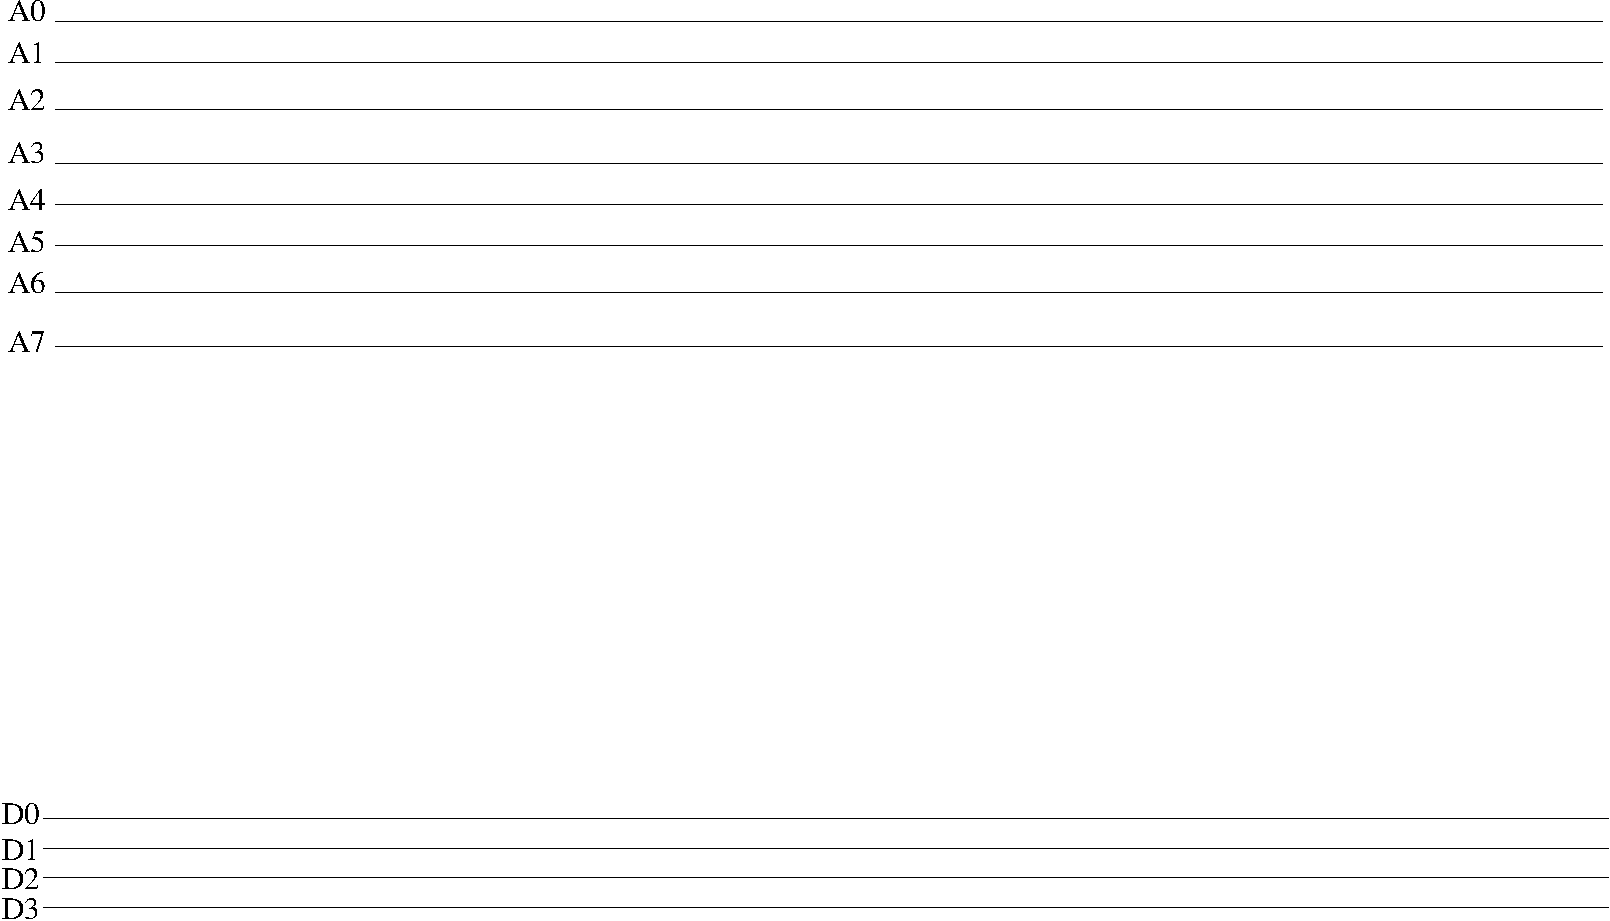
\includegraphics[width=0.7\textwidth]{memoria}
 \caption{Barramento de 8 bits da endereço e de 4 bits para dados}
 \label{fig:memoria}
\end{figure}


\questao{A figura abaixo apresenta um barramento de endereço de 8 bits $A0-A7$ e barramento de dados de 8 bits $D0-D7$.} Deseja-se utilizar CIs de  memória de
128x8 para construir uma memória de 256x8. Desenhe os CIs de memória e mostre como os mesmos devem ser ligados ao barramento e quais são os circuitos ou portas
lógicas necessários para obter a solução do problema.


\begin{figure}[H]
 \centering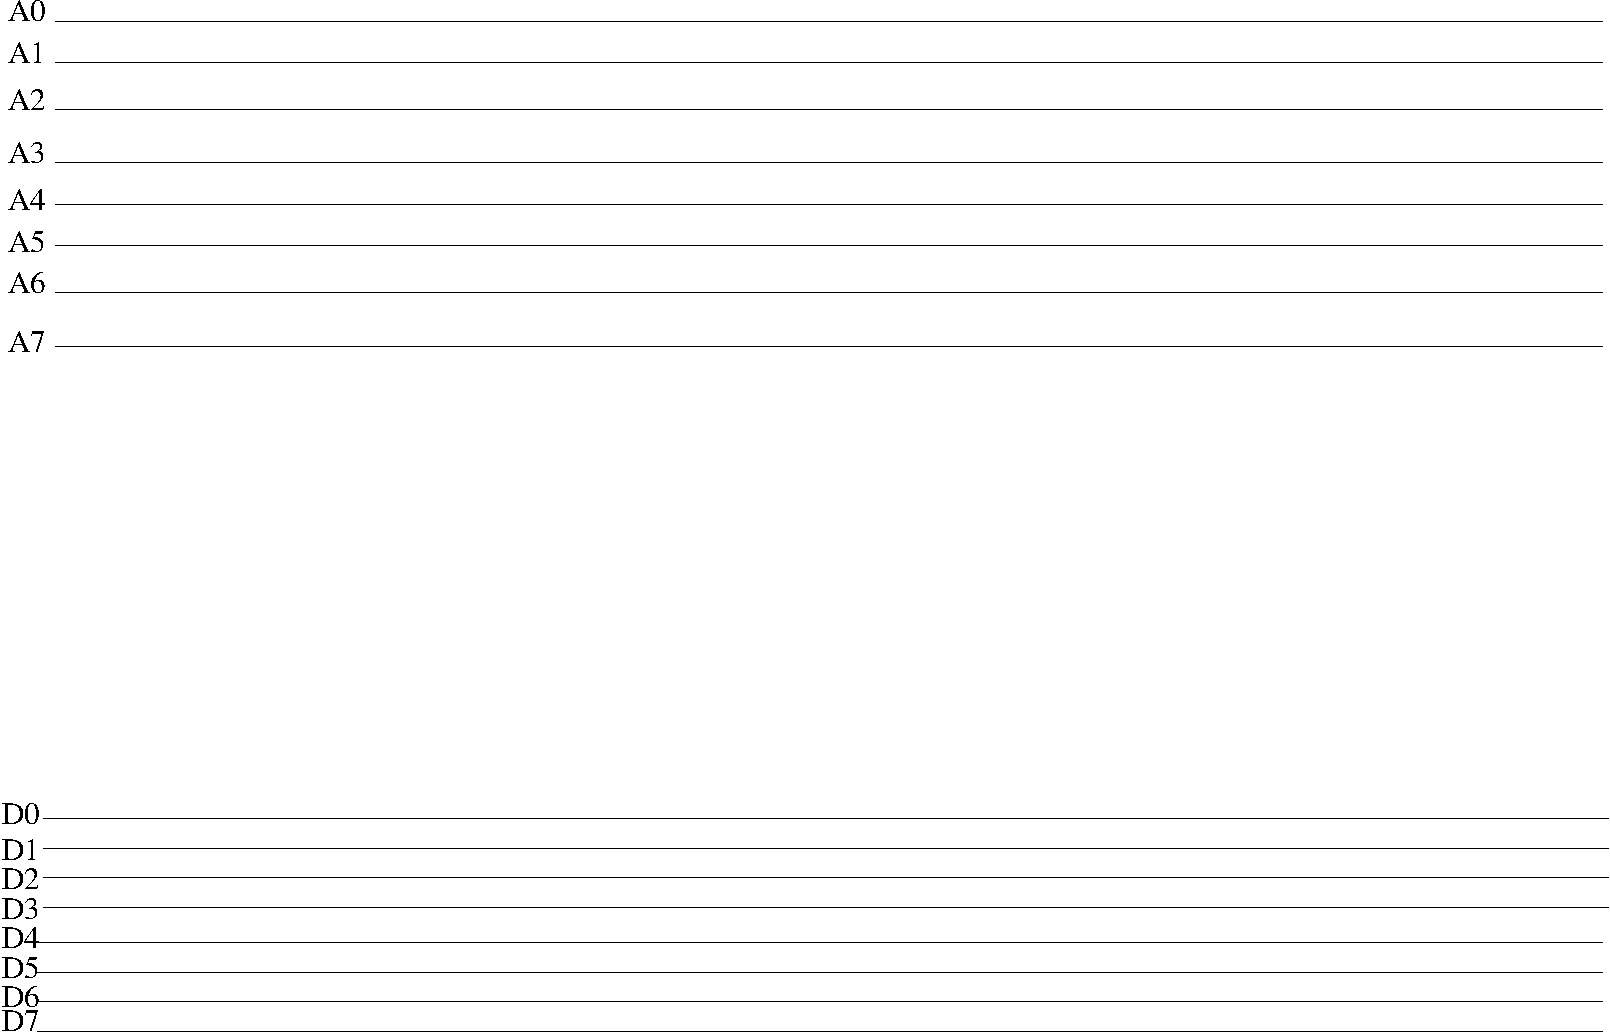
\includegraphics[width=0.7\textwidth]{memoria2}
 \caption{Barramento de 8 bits da endereço e de 8 bits para dados}
 \label{fig:memoria2}
\end{figure}


\questao{A figura abaixo apresenta um diagrama de endereços de um certo computador. Existem diferentes faixas de endereços e nestas faixas de encdereços apenas
um CHIP de memória está sendo acessado.} Desenhos os diversos chips de memória envolvidos e conecte os CS de cada um destes para que funcionem apenas dentro da
faixa de endereços como na figura. Represente a quantidade de linhas para o barramento de dados e de endereços e todos os circuitos necessários para ativar os
pinos de CS de cada um dos chips de memória.


\begin{figure}[H]
 \centering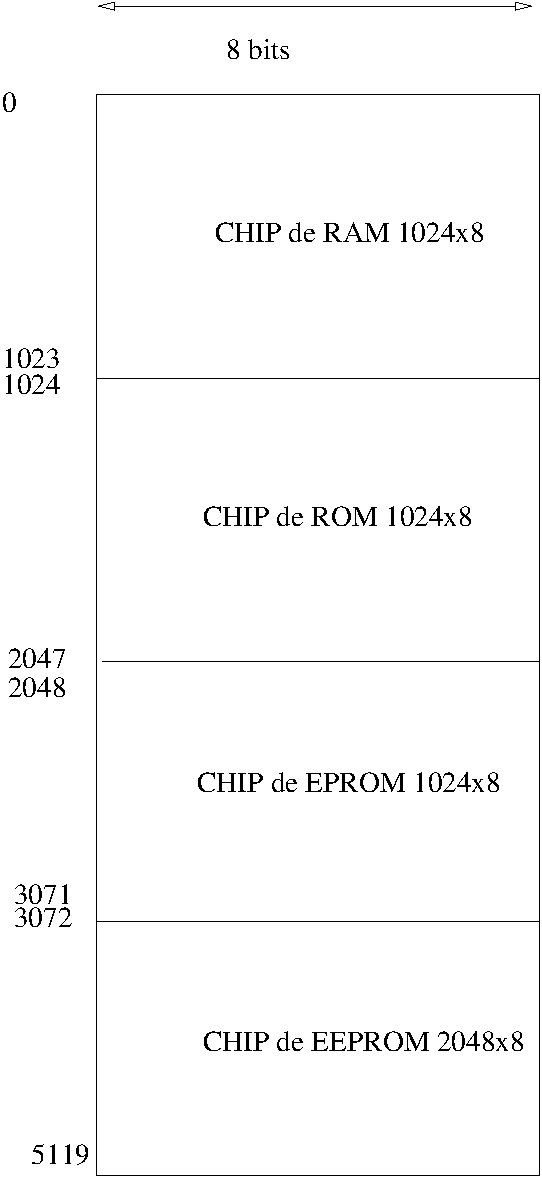
\includegraphics[width=0.3\textwidth]{memoria3}
 \caption{Memória de um computador X}
 \label{fig:memoria3}
\end{figure}


\questao{A figura abaixo mostra uma memória do tipo PROM com fusíveis. A memória possui apenas duas linhas de endereço. Mostre como seria a memória caso a mesma
tenha sido gravada para representar os dados abaixo}

\begin{figure}[H]
 \centering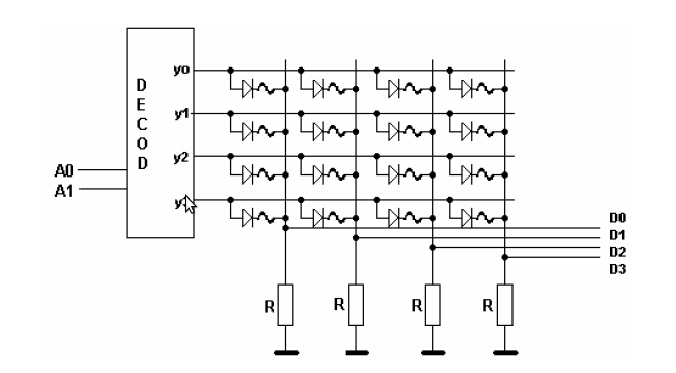
\includegraphics[width=0.3\textwidth]{prom}
 \caption{Diagrama interno de uma PROM com fusíveis}
 \label{fig:prom}
\end{figure}

\begin{verbatim}
Endereco 0: 1 1 1 1
Endereco 1: 1 0 1 0
Endereco 2: 1 1 0 0
Endereco 3: 0 0 1 1
\end{verbatim}

\questao{O CHIP 2125A é uma RAM estática de 1Kx1 de capacidade com entrada de dados independe da saída de dados. (Diagrama abaixo)}. Mostre como conectar esta
memória para formar um módulo de 1Kx8.


\begin{figure}[H]
 \centering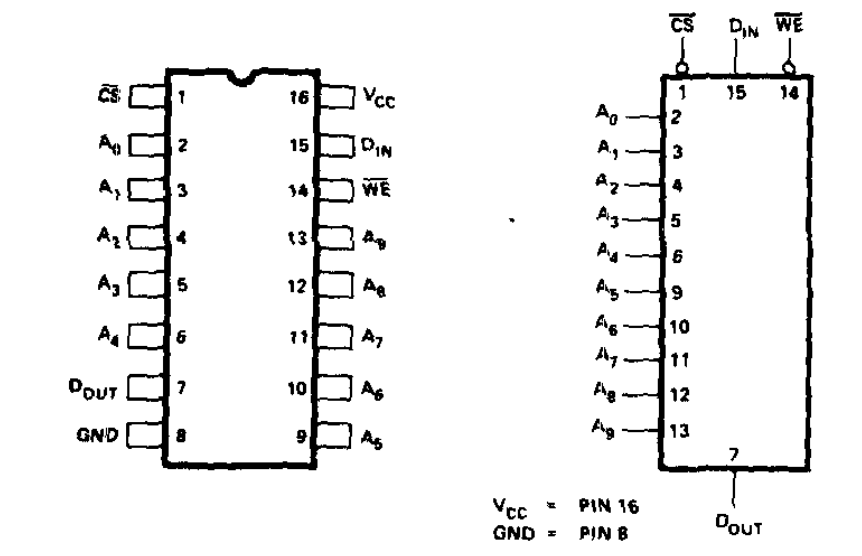
\includegraphics[width=0.3\textwidth]{2125a}
 \caption{Chip RAM 2125}
 \label{fig:2125}
\end{figure}

\questao{A figura abaixo mostra um programador de EPROM manual, explique como este funciona.}

\begin{figure}[H]
 \centering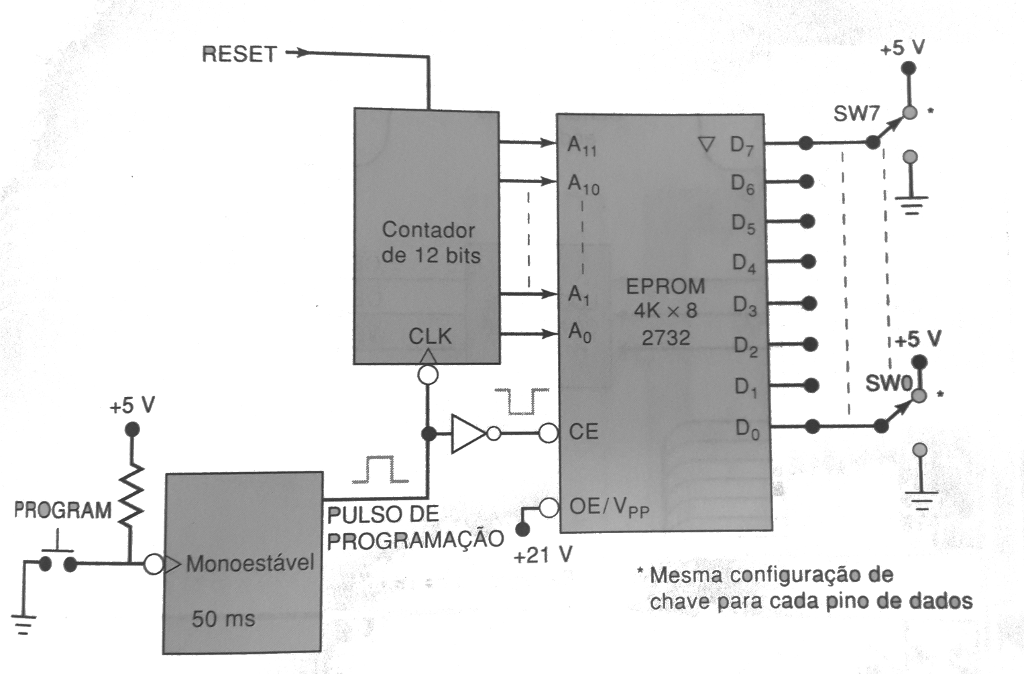
\includegraphics[width=0.3\textwidth]{programador}
 \caption{Programador de Eprom}
 \label{fig:programador}
\end{figure}


\questao{Outra aplicação de uma ROM é a geração de sinais de temporização e controle. A figura abaixo mostra uma ROM com um gerador de enderecos. Assumindo que o
conteudo da ROM é o indicado na tabela abaixo, desenhe o diagrama de ondas em cada saída da ROM. }

\begin{figure}[H]
 \centering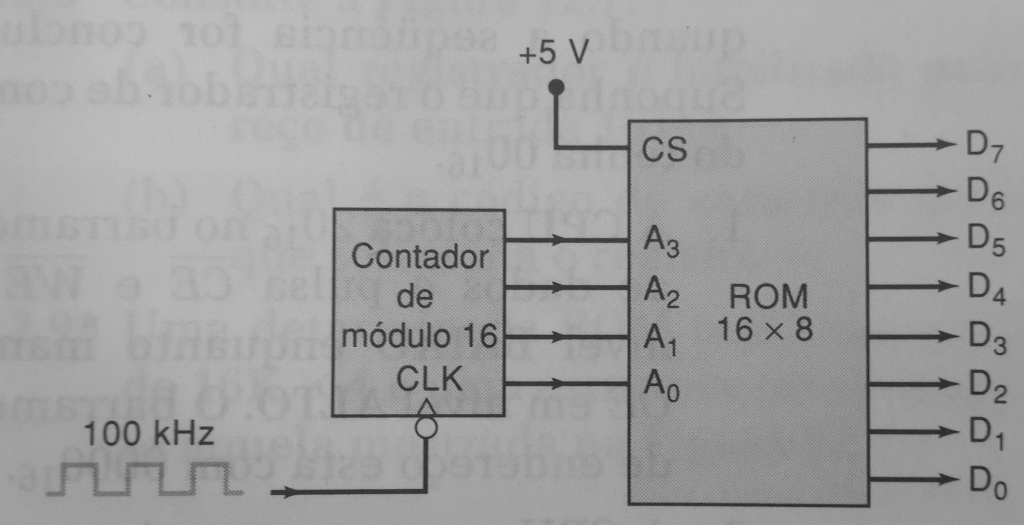
\includegraphics[width=0.3\textwidth]{ondas}
 \caption{Outro uso para ROM}
 \label{fig:outro}
\end{figure}

\begin{figure}[H]
 \centering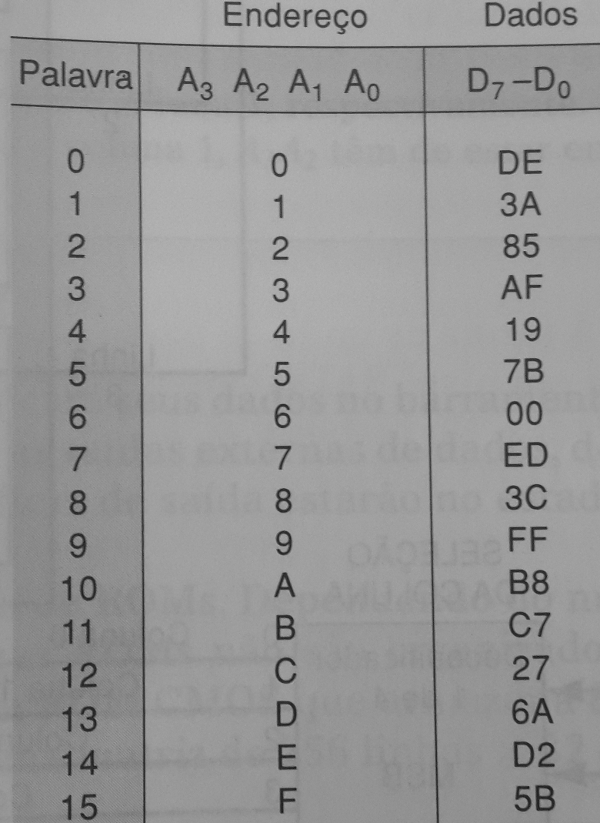
\includegraphics[width=0.3\textwidth]{conteudo}
 \caption{Conteúdo da ROM}
 \label{fig:conteudo}
\end{figure}


\questao{SIMULAÇÃO: Utilizando o Proteus ISIS, teste o funcionamento do CHIP de memória ram estática 62256. Use chaves ou mesmo um microcontrolador para setar
valores nos barramentos de dados e de endereços. Crie uma operação de escrita e de leitura.}

\end{document}